% Q5: 5G Link Budget Block Diagram
% Teaching diagram: visual representation of the Friis equation
\documentclass[border=10pt]{standalone}
\usepackage{tikz}
\usepackage{amsmath}
\usetikzlibrary{arrows.meta, positioning, shapes.geometric, decorations.pathreplacing}

\renewcommand{\familydefault}{\sfdefault}

\begin{document}
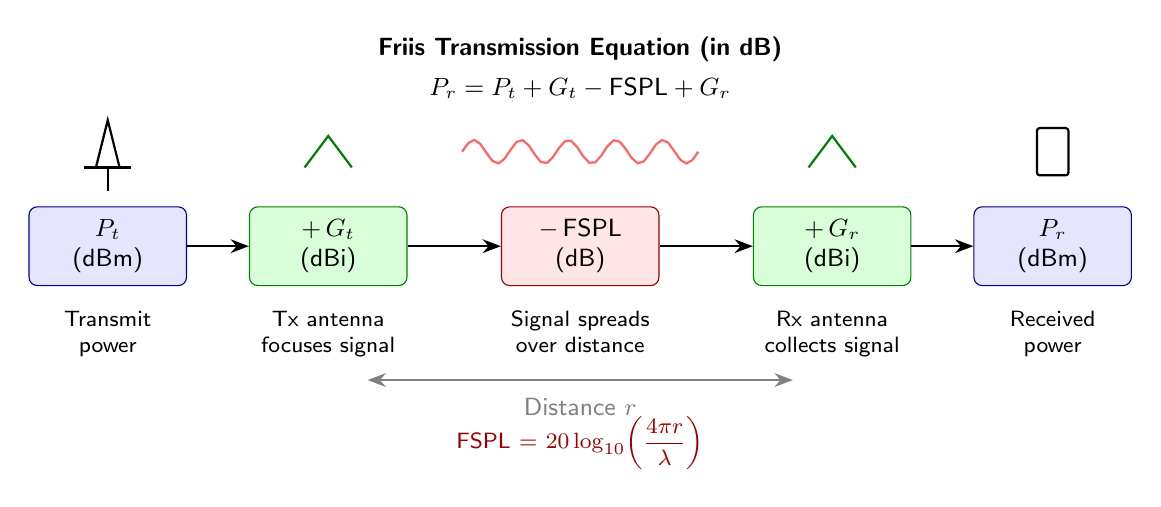
\begin{tikzpicture}[
    every node/.style={font=\sffamily\normalsize},
    >=Stealth,
    block/.style={draw, rounded corners=3pt, minimum width=2cm, minimum height=1cm, align=center, font=\sffamily\small},
    gain/.style={block, fill=green!15, draw=green!50!black},
    loss/.style={block, fill=red!10, draw=red!60!black},
    power/.style={block, fill=blue!10, draw=blue!60!black},
]

% --- Title ---
\node[font=\sffamily\small\bfseries] at (6, 4.5) {Friis Transmission Equation (in dB)};
\node[font=\sffamily\small] at (6, 4.0) {$P_r = P_t + G_t - \text{FSPL} + G_r$};

% --- Blocks ---
\node[power] (pt) at (0, 2) {$P_t$\\(dBm)};
\node[gain] (gt) at (2.8, 2) {$+\,G_t$\\(dBi)};
\node[loss] (fspl) at (6, 2) {$-\,$FSPL\\(dB)};
\node[gain] (gr) at (9.2, 2) {$+\,G_r$\\(dBi)};
\node[power] (pr) at (12, 2) {$P_r$\\(dBm)};

% --- Arrows ---
\draw[->, thick] (pt) -- (gt);
\draw[->, thick] (gt) -- (fspl);
\draw[->, thick] (fspl) -- (gr);
\draw[->, thick] (gr) -- (pr);

% --- Physical meaning labels ---
\node[below, font=\sffamily\footnotesize, text width=1.8cm, align=center] at (0, 1.3) {Transmit\\power};
\node[below, font=\sffamily\footnotesize, text width=1.8cm, align=center] at (2.8, 1.3) {Tx antenna\\focuses signal};
\node[below, font=\sffamily\footnotesize, text width=2.2cm, align=center] at (6, 1.3) {Signal spreads\\over distance};
\node[below, font=\sffamily\footnotesize, text width=1.8cm, align=center] at (9.2, 1.3) {Rx antenna\\collects signal};
\node[below, font=\sffamily\footnotesize, text width=1.8cm, align=center] at (12, 1.3) {Received\\power};

% --- Icons ---
% Base station tower
\draw[thick] (-0.15, 3.0) -- (0, 3.6) -- (0.15, 3.0);
\draw[thick] (-0.3, 3.0) -- (0.3, 3.0);
\draw[thick] (0, 3.0) -- (0, 2.7);
% Antenna gain (Tx)
\draw[thick, green!50!black] (2.5, 3.0) -- (2.8, 3.4) -- (3.1, 3.0);
% Free space (wave)
\draw[thick, red!60, domain=4.5:7.5, samples=40] plot (\x, {3.2 + 0.15*sin(360*(\x-4.5)/0.6)});
% Antenna gain (Rx)
\draw[thick, green!50!black] (8.9, 3.0) -- (9.2, 3.4) -- (9.5, 3.0);
% Phone icon
\draw[thick, rounded corners=1pt] (11.8, 2.9) rectangle (12.2, 3.5);

% --- Distance annotation ---
\draw[<->, thick, gray] (3.3, 0.3) -- (8.7, 0.3);
\node[below, font=\sffamily\small, gray] at (6, 0.2) {Distance $r$};

% --- FSPL formula (without revealing distance-doubling answer) ---
\node[font=\sffamily\footnotesize, red!60!black, text width=3.5cm, align=center] at (6, -0.5)
    {$\text{FSPL} = 20\log_{10}\!\left(\dfrac{4\pi r}{\lambda}\right)$};

\end{tikzpicture}
\end{document}
